\documentclass[11pt,a4paper]{scrartcl}
\usepackage[T1]{fontenc}
\usepackage[utf8]{inputenc}
\usepackage[ngerman]{babel}
\usepackage{microtype}
\usepackage{lmodern}
\usepackage{amsmath}
\usepackage{amsfonts}
\usepackage{amssymb}
\usepackage{enumerate}
\usepackage{graphicx}

\begin{document}

\author{Johannes Merkle\\Ralf Vogler}
\title{Query Optimization}
\subtitle{1. Exercise}

\maketitle

\section*{Exercise 1}
Tinydb implementation in file Exercise1.java
\subsubsection*{Part 1}
Find all students that attended the lectures together with Schopenhauer, excluding
Schopenhauer himself.
\begin{verbatim}
SELECT s2.name FROM studenten s1, studenten s2, hoeren h1, hoeren h2
WHERE s1.name='Schopenhauer' AND s1.matrnr=h1.matrnr AND s2.matrnr=h2.matrnr
AND h1.vorlnr=h2.vorlnr AND s2.matrnr<>s1.matrnr
\end{verbatim}
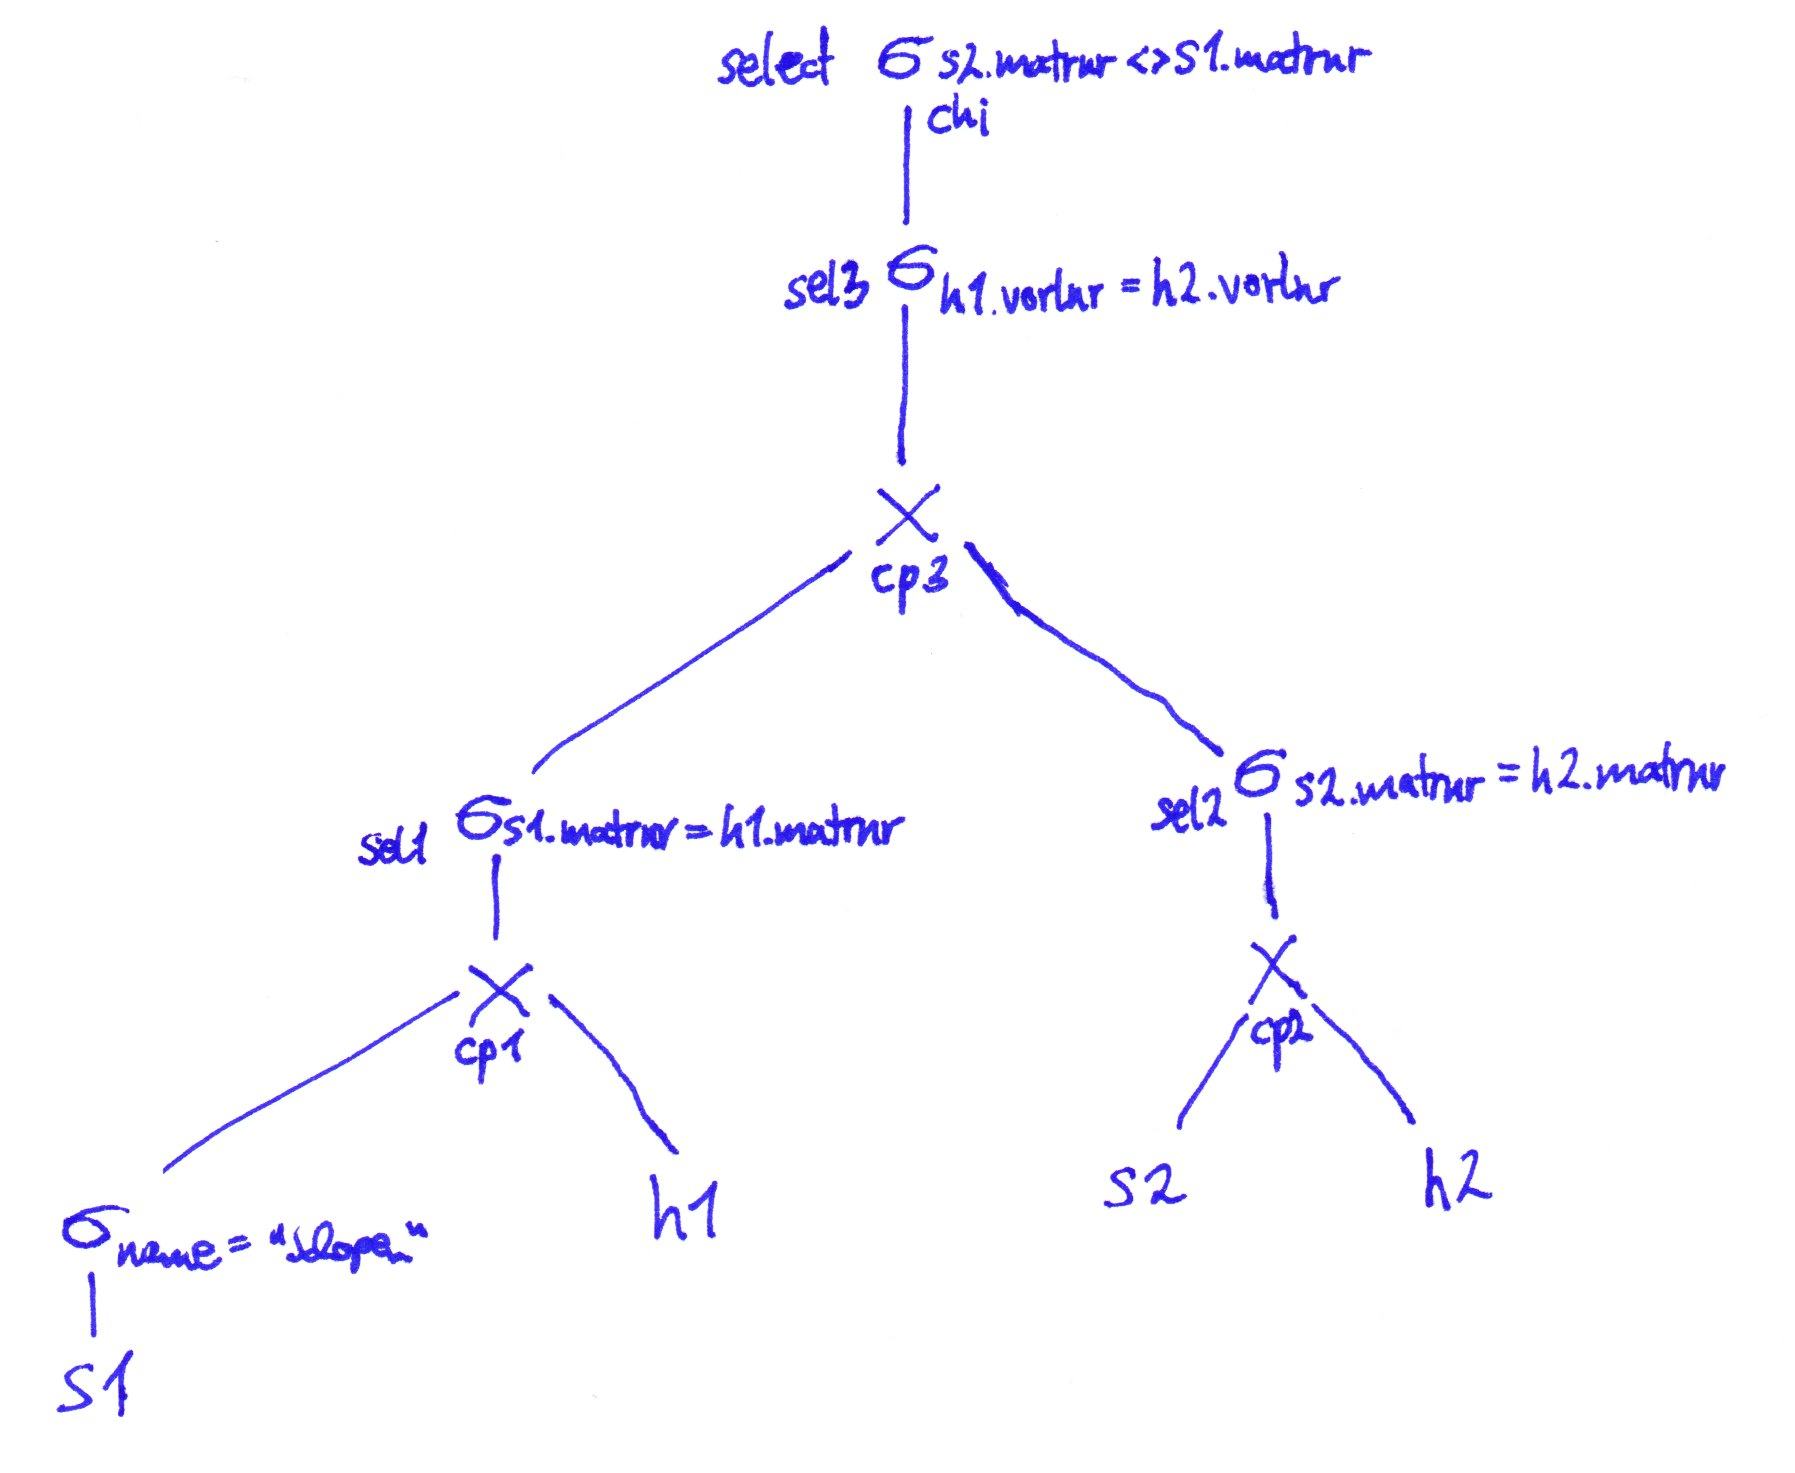
\includegraphics[scale=.17]{part1.jpg}
\subsubsection*{Part 2}
Find all professors whose lectures attended at least two students.
\begin{verbatim}
SELECT p.name, COUNT(h.matrnr) AS hoerer FROM professoren p, vorlesungen v, hoeren h
WHERE p.persnr=v.gelesenvon AND v.vorlnr=h.vorlnr
GROUP BY p.name
HAVING COUNT(h.matrnr)>=2
\end{verbatim}
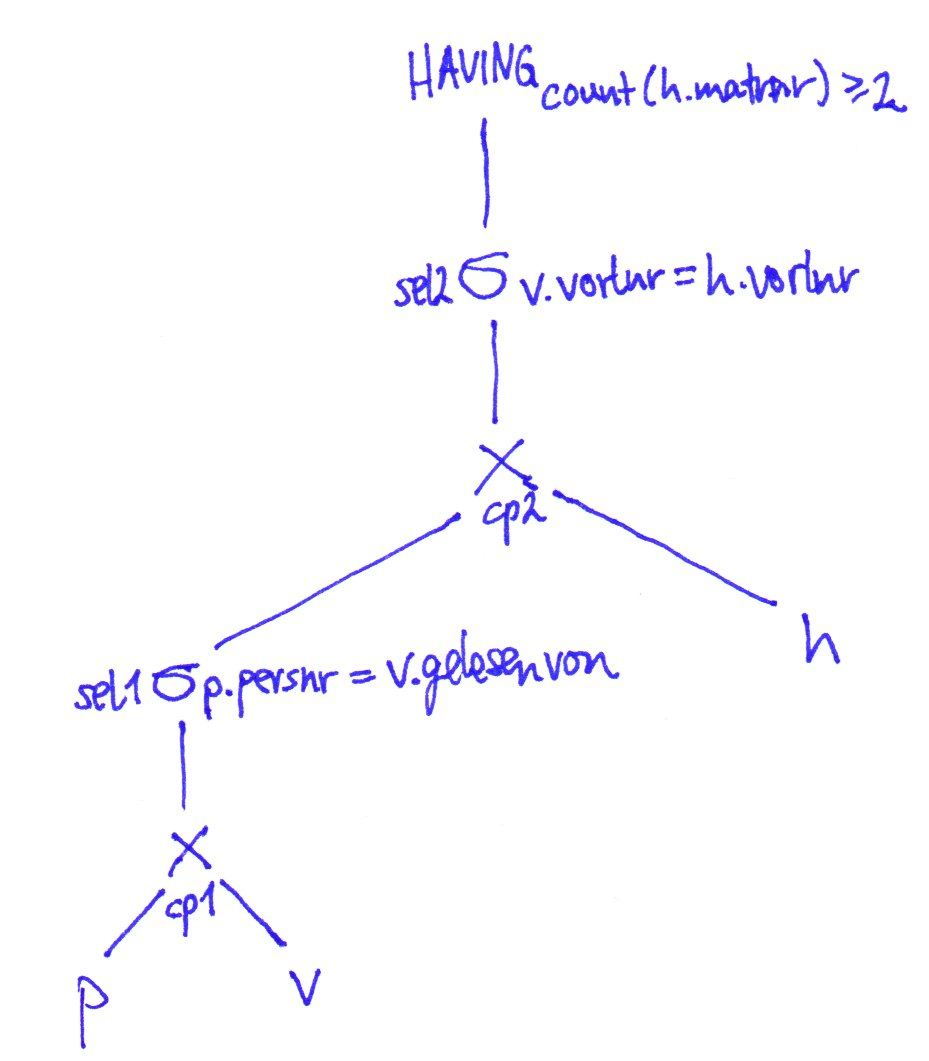
\includegraphics[scale=1]{part2a.jpg}\\
We implemented a having clause because it is flexible if the number should change.
The alternative would be to use the relation hoeren two times:
\begin{verbatim}
SELECT p.name FROM professoren p, vorlesungen v, hoeren h1, hoeren h2
WHERE p.persnr=v.gelesenvon AND v.vorlnr=h1.vorlnr AND v.vorlnr=h2.vorlnr
AND h1.matrnr<>h2.matrnr
\end{verbatim}
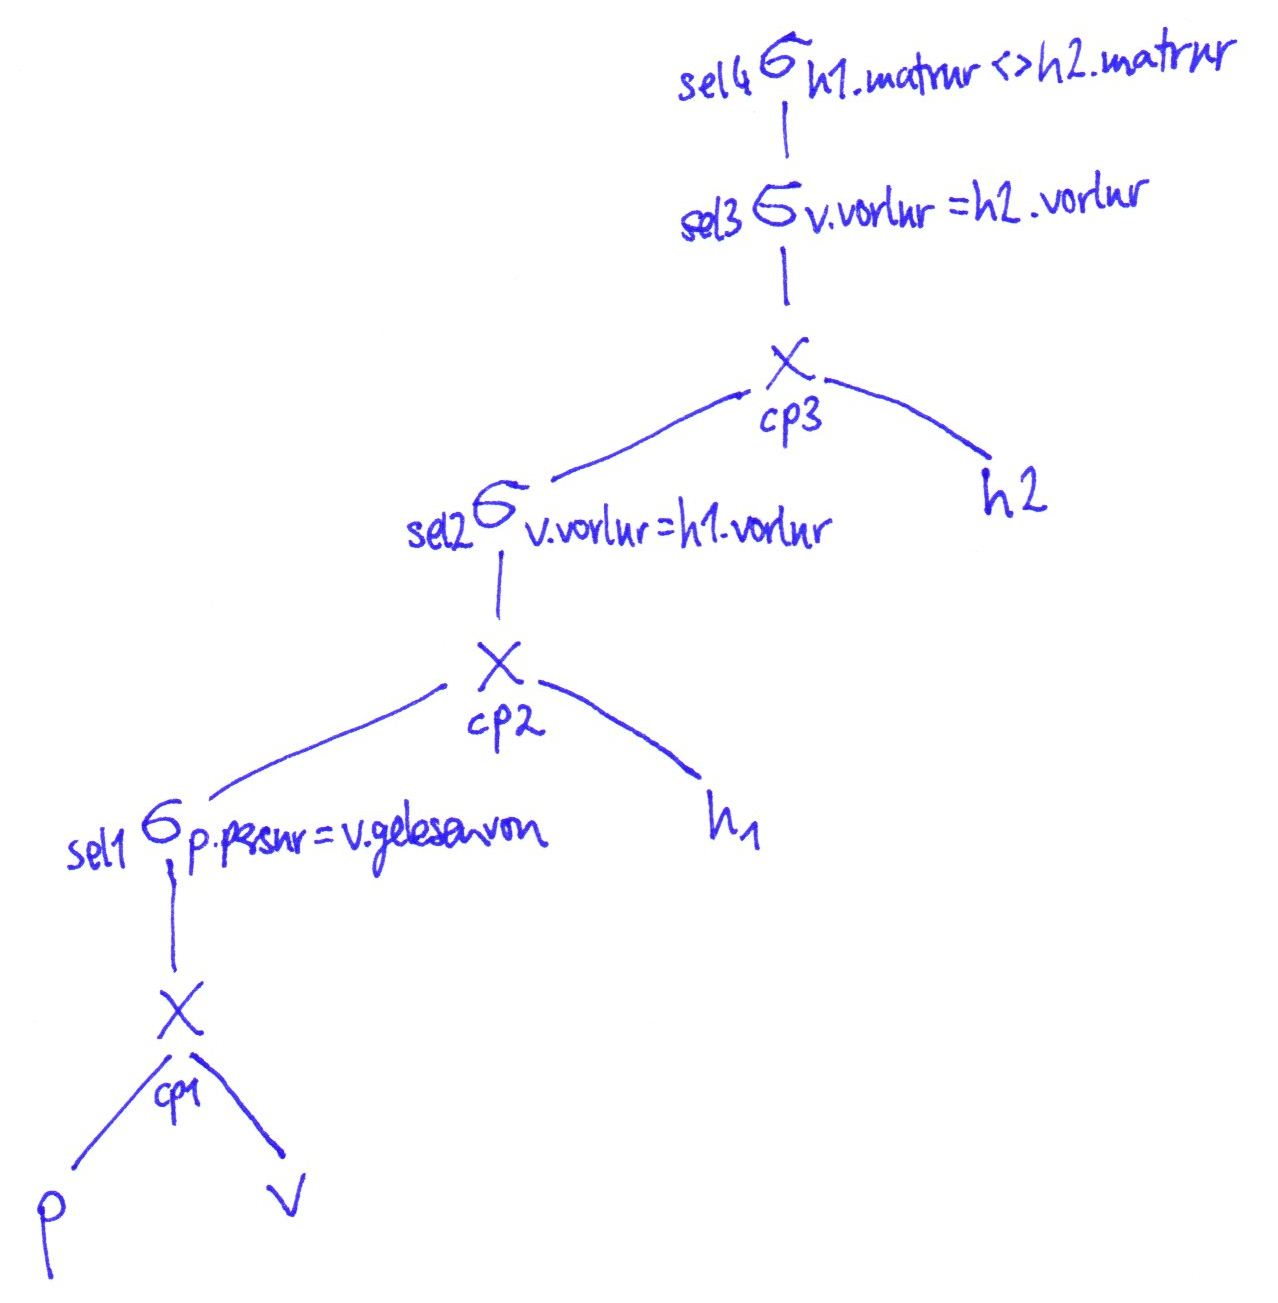
\includegraphics[scale=1]{part2b.jpg}


\section*{Exercise 2}
Tinydb implementation in file Exercise2.java

\end{document}
